\chapter*{Opinión del tutor}

\begin{figure}[H]
 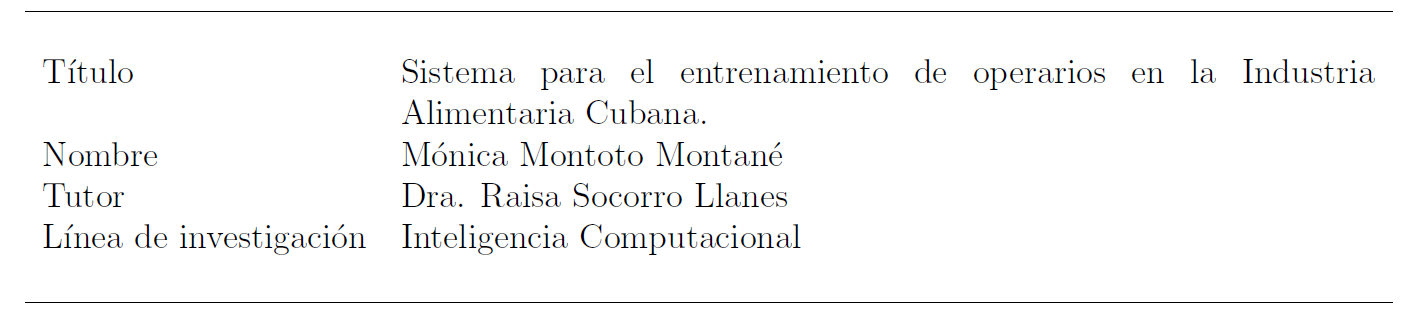
\includegraphics[width=1\linewidth]{imagen/opinion.png}
\end{figure}

La Industria Alimentaria Cubana se caracteriza por poseer jornadas laborales ininterrumpidas y un personal que cambia frecuentemente. Este flujo constante de trabajo y personal no garantiza la permanencia en cada puesto de trabajo de un personal altamente capacitado y además dificulta el proceso de capacitación.

El Instituto de Investigación de la Industria Alimentaria (IIIA), junto con las facultades de Ingeniería Química e Ingeniería Informática de la Universidad Tecnológica de La Habana (CUJAE), desarrolló dos aplicaciones informáticas: un Sistema Generador de Bases de Conocimiento (SGBC) y un Sistema Experto para el Control de Procesos Químicos (SECPROIT).
El primero genera bases de conocimiento que contienen la información referente a los procesos productivos que pueden ocurrir en una fábrica. El segundo, se utiliza para producir entrenamientos y capacitar a los operarios de la fábrica. A partir de estos sistemas, se pueden capacitar a los trabajadores en los procesos productivos que maniobran y se reducir los riesgos de errores por desconocimiento. En las pruebas realizadas a SECPROIT se detectaron un conjunto de no conformidades que aplazaron su despliegue en la industrias.

El trabajo presentado por la estudiante presenta una nueva versión donde se solucionan estas no conformidades y se incorporan nuevas funcionalidades.

Para el desarrollo de este trabajo la estudiante tuvo aplicar los conocimientos adquiridos durante la carrera y profundizar en otros temas que no fueron abordados directamente en la misma. Implicó un estudio del estado del arte vinculado a esta temática, consultando una bibliografía en idioma inglés y profundizando además en modelos para la evaluación del aprendizaje.

Es importante destacar que durante el desarrollo de este trabajo la estudiante demostró un alto grado de independencia, creativa, disciplina y disposición al trabajo. La distancia impuesta por la situación epidemiológica en el país en los comienzos de este trabajo no afectó , nunca ha sido una traba para su trabajo, reportando sus avances y tropiezos. También reconocer que desde el inicio del trabajo a finales de 2do año ha contribuido con la alfabetización informática del usuario final, con manuales de usuario y asesoría técnica, incluso para otras aplicaciones vinculadas al campo de acción del usuario.

También es importante destacar como la estudiante que llegó a 2do año con dos arrastres de Matemática 1 y 2, defiende hoy en el primer grupo de estudiantes de su año con excelente trabajo, y que además supo combinar estudios,13 de Marzo, Festival de Cultura, Jornada Científica entre otras tareas.

Los resultados obtenidos en el trabajo cumplen con los objetivos trazados, por lo que considero que en función a las respuestas del estudiante a las preguntas del tribunal, Mónica Montoto Montané puede aspirar a la calificación de EXCELENTE (5 puntos).

\vspace{1.5cm}

Tutora:

\vspace{1.5cm}
\begingroup	
\setlength{\tabcolsep}{10pt} % Default value: 6pt
\renewcommand{\arraystretch}{0.5} % Default value: 1

\begin{tabular}{c}
	
\includegraphics[width=0.2\textwidth]{imagen/raisa.png}\\
	\noindent\rule{6cm}{0.4pt}\\
	Dra. Raisa Socorro Llanes \\
	\\
	Profesora Auxiliar 
\end{tabular}
\endgroup

\vspace{1.5cm}
Facultad de Ingeniería Informática

Universidad Tecnológica de la Habana 

CUJAE, La Habana, Cuba, 9 de diciembre de 2022